\documentclass[12pt]{article}

\usepackage[english]{babel}
\usepackage[utf8]{inputenc}
\usepackage{amsmath}
\usepackage{commath}
\usepackage{booktabs}
\usepackage[alf]{abntex2cite}
\usepackage{indentfirst}
\usepackage{graphicx}
\usepackage{multicol,lipsum}
\usepackage{geometry}
\usepackage[alf]{abntex2cite}
\usepackage{siunitx}
\usepackage{subfigure}
\graphicspath{{../../Figures/Report_19_09/}{../../Images/Report_19_09/}}

\geometry{
  paper = a4paper,
  inner = 3cm,
  outer = 3cm,
  top = 2cm,
  bottom = 2cm
}

\usepackage{tabularx}

\begin{document}
%\maketitle

\onehalfspacing

\begin{titlepage}
\begin{center}

\Huge{Universidade Federal de Alagoas}\\
\large{Instituto de Computação}\\ 
\large{Laboratório de Computação Científica e Análise Numérica}\\ 
\vspace{220pt}
\textbf{\LARGE{Research report}}\\
%\title{{\large{Título}}}
\vspace{3,5cm}
\end{center}

\begin{flushleft}
\begin{tabbing}
Student: Danilo Fernandes Costa\\
Professor: Alejandro Frery\\
\end{tabbing}
\end{flushleft}
\vspace{1cm}

\begin{center}
\vspace{\fill}
September\\
2019
\end{center}
\end{titlepage}

\section{Introduction}

In this report, we show results of the analysis of samples from plantation regions observed over time.
%%% ACF Me parece que siunitx ajuda formatar datas, mas eu nunca o fiz
The first observation was made on 16 May 2016, which was followed by four others at time intervals of 24 days. 
Those regions consist of three soybeans crops, three wheat, two oats, and two canola and are shown in Figs.~\ref{fig:r1} to~\ref{fig:r5}. 
Those samples were obtained using the classification of the regions given in Fig.~\ref{fig:classes}.
%%% ACF Como foi obtida essa classificação
%%% DFC Debanshu enviou-me a classificação das regiões junto com o dataset

We fit the Beta distribution to histograms of the distances of the samples to the trihedral and random volume scatterers. 
In addition, we perfor the Kolmogorov-Smirnov good-of-fit test to verify the quality of the fit. 
These scatterers were chosen because they were more sensitive to vegetation variation in the analyzed regions, as can be verified in the Figs.~\ref{fig:tp} and~\ref{fig:rvp} which contain, respectively, the pixel proportions in the sample that is more similar to the trihedral and the random volume as a function of time.

\begin{figure}[hbt]
\centering
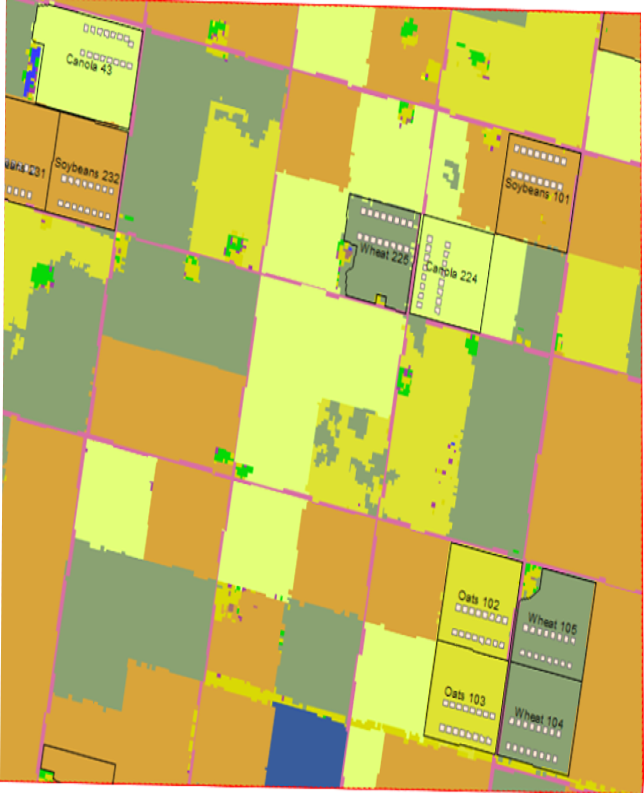
\includegraphics[width = .55\linewidth]{/Regions/classes}
\label{fig:classes}
\caption{Classification of the regions on the PolSAR image}
\end{figure}

\begin{figure*}[hbt]
\centering
\subfigure[1th observation\label{fig:r1}]{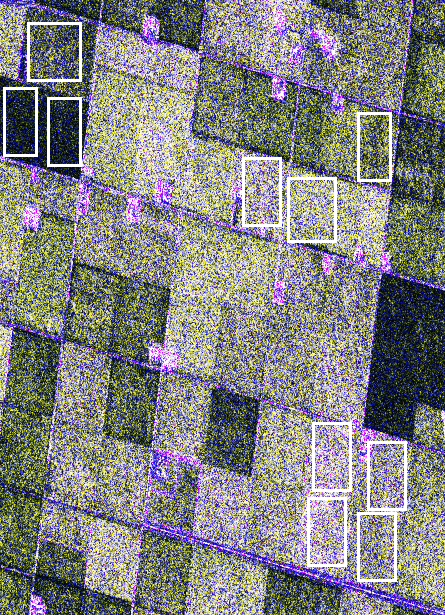
\includegraphics[width = .32\linewidth]{/Regions/regions_1}}
\subfigure[2th observation\label{fig:r2}]{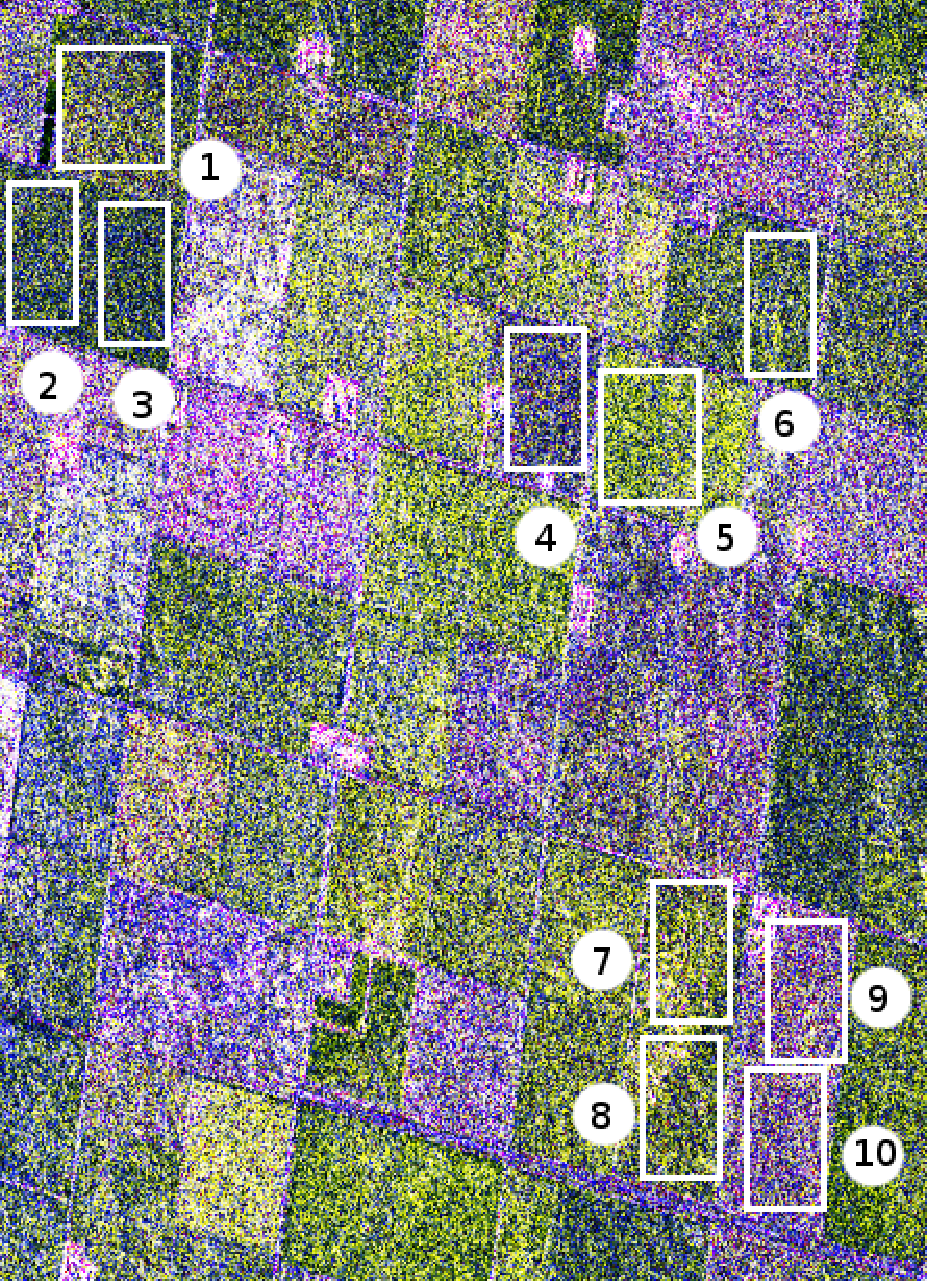
\includegraphics[width = .32\linewidth]{/Regions/regions_2}}
\subfigure[3th observation\label{fig:r3}]{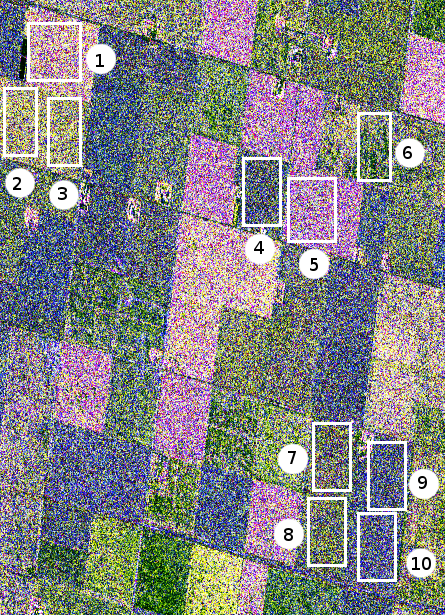
\includegraphics[width = .32\linewidth]{/Regions/regions_3}}
\subfigure[4th observation\label{fig:r4}]{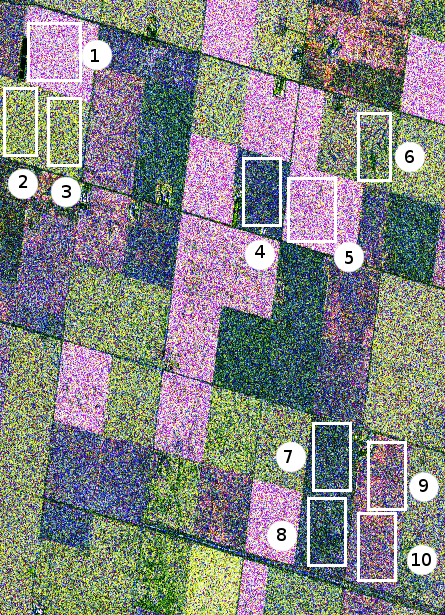
\includegraphics[width = .32\linewidth]{/Regions/regions_4}}
\subfigure[5th observation\label{fig:r5}]{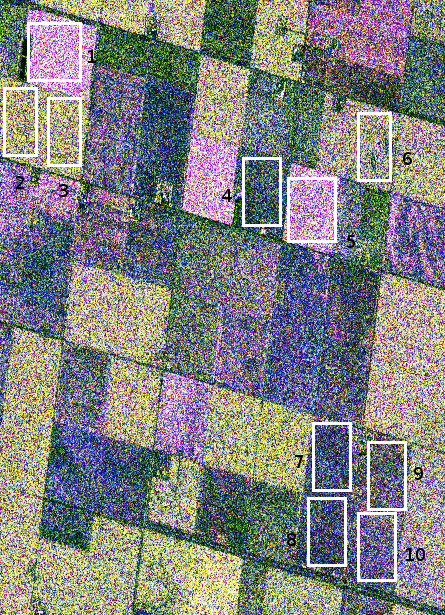
\includegraphics[width = .32\linewidth]{/Regions/regions_5}}
\caption{Samples analyzed over time: 1 to 10 corresponding, respectively, to Canola 43, Soybeans 231, Soybeans 232, Wheat 225, Canola 224, Soybeans 101, Oats 102, Oats 103, Wheat 105 and Wheat 104}
\label{fig:regions}
\end{figure*}

\begin{figure*}[hbt]
\centering
\subfigure[Trihedral\label{fig:tp}]{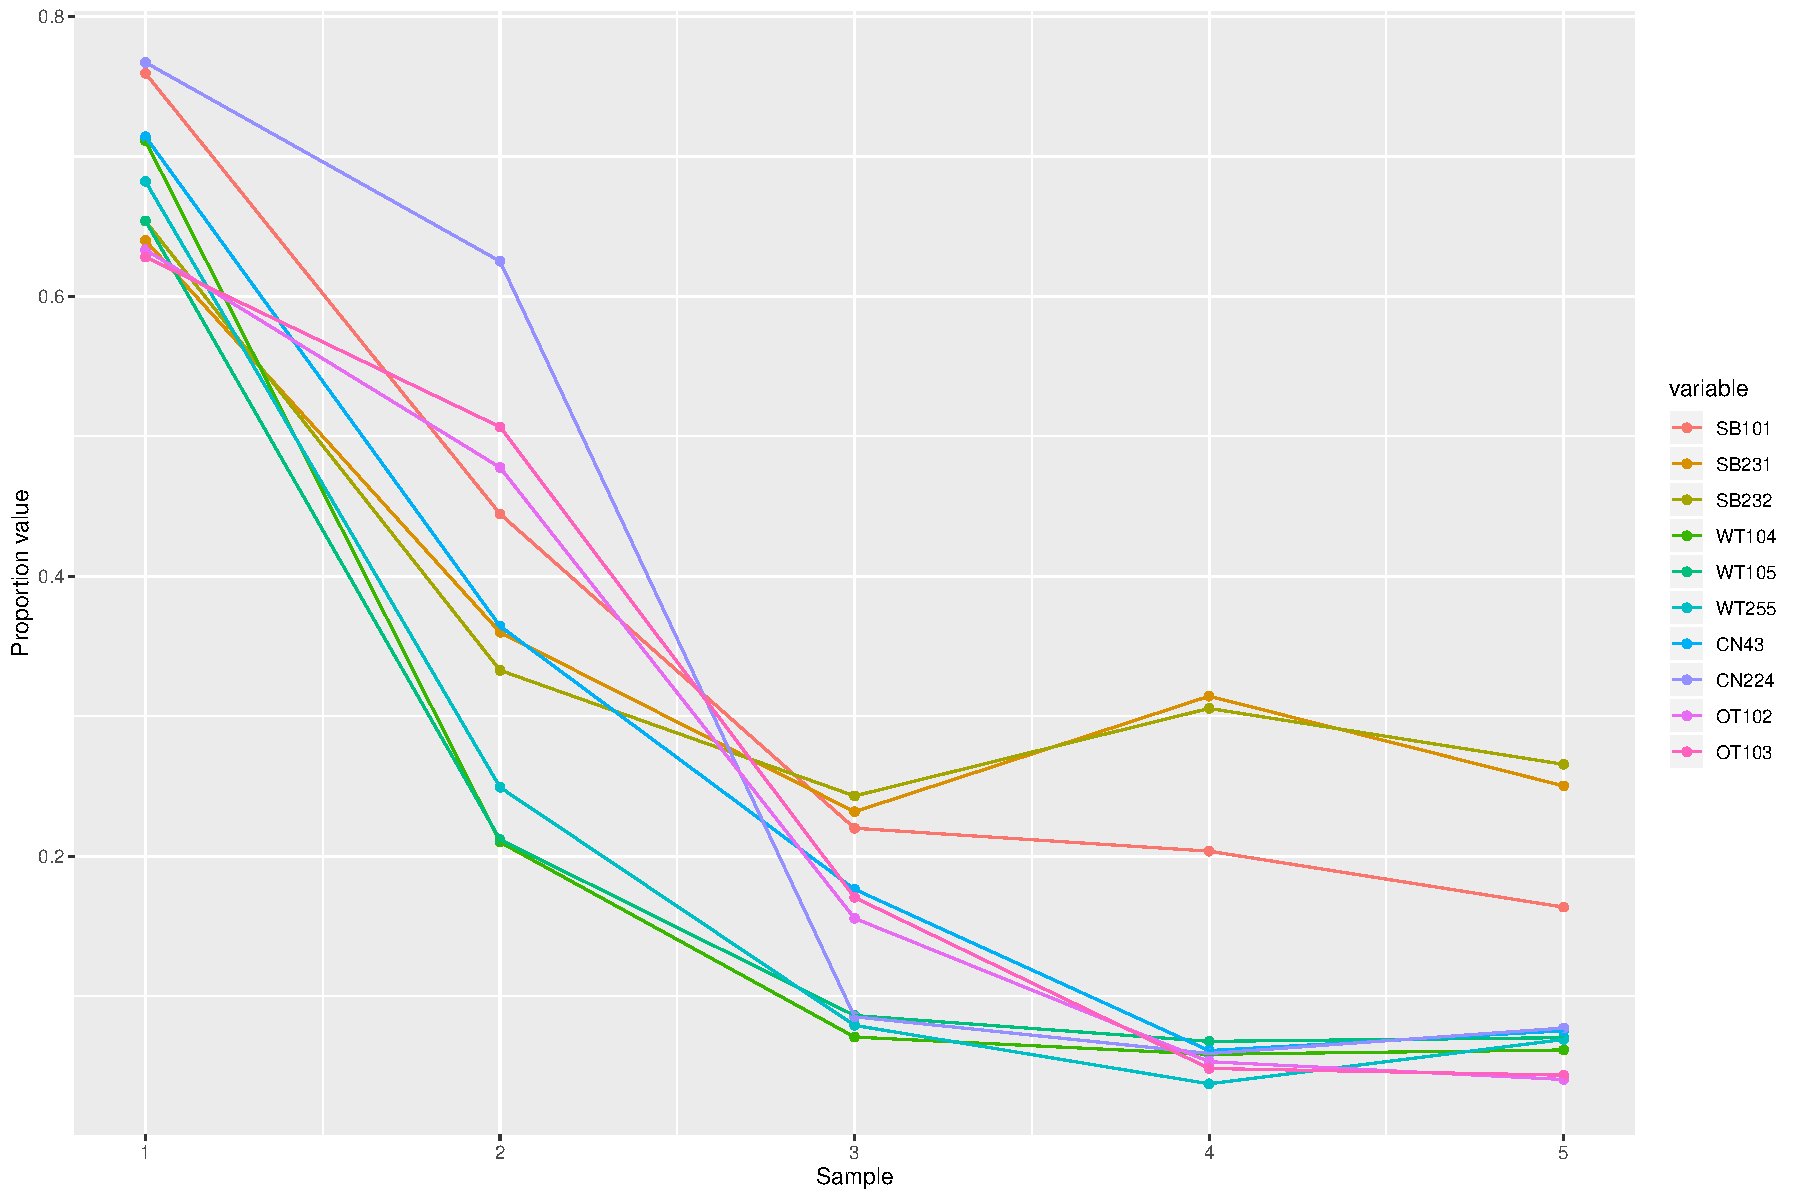
\includegraphics[width = .49\linewidth]{/Parameters/tri_proportion}}
\subfigure[Random Volume\label{fig:rvp}]{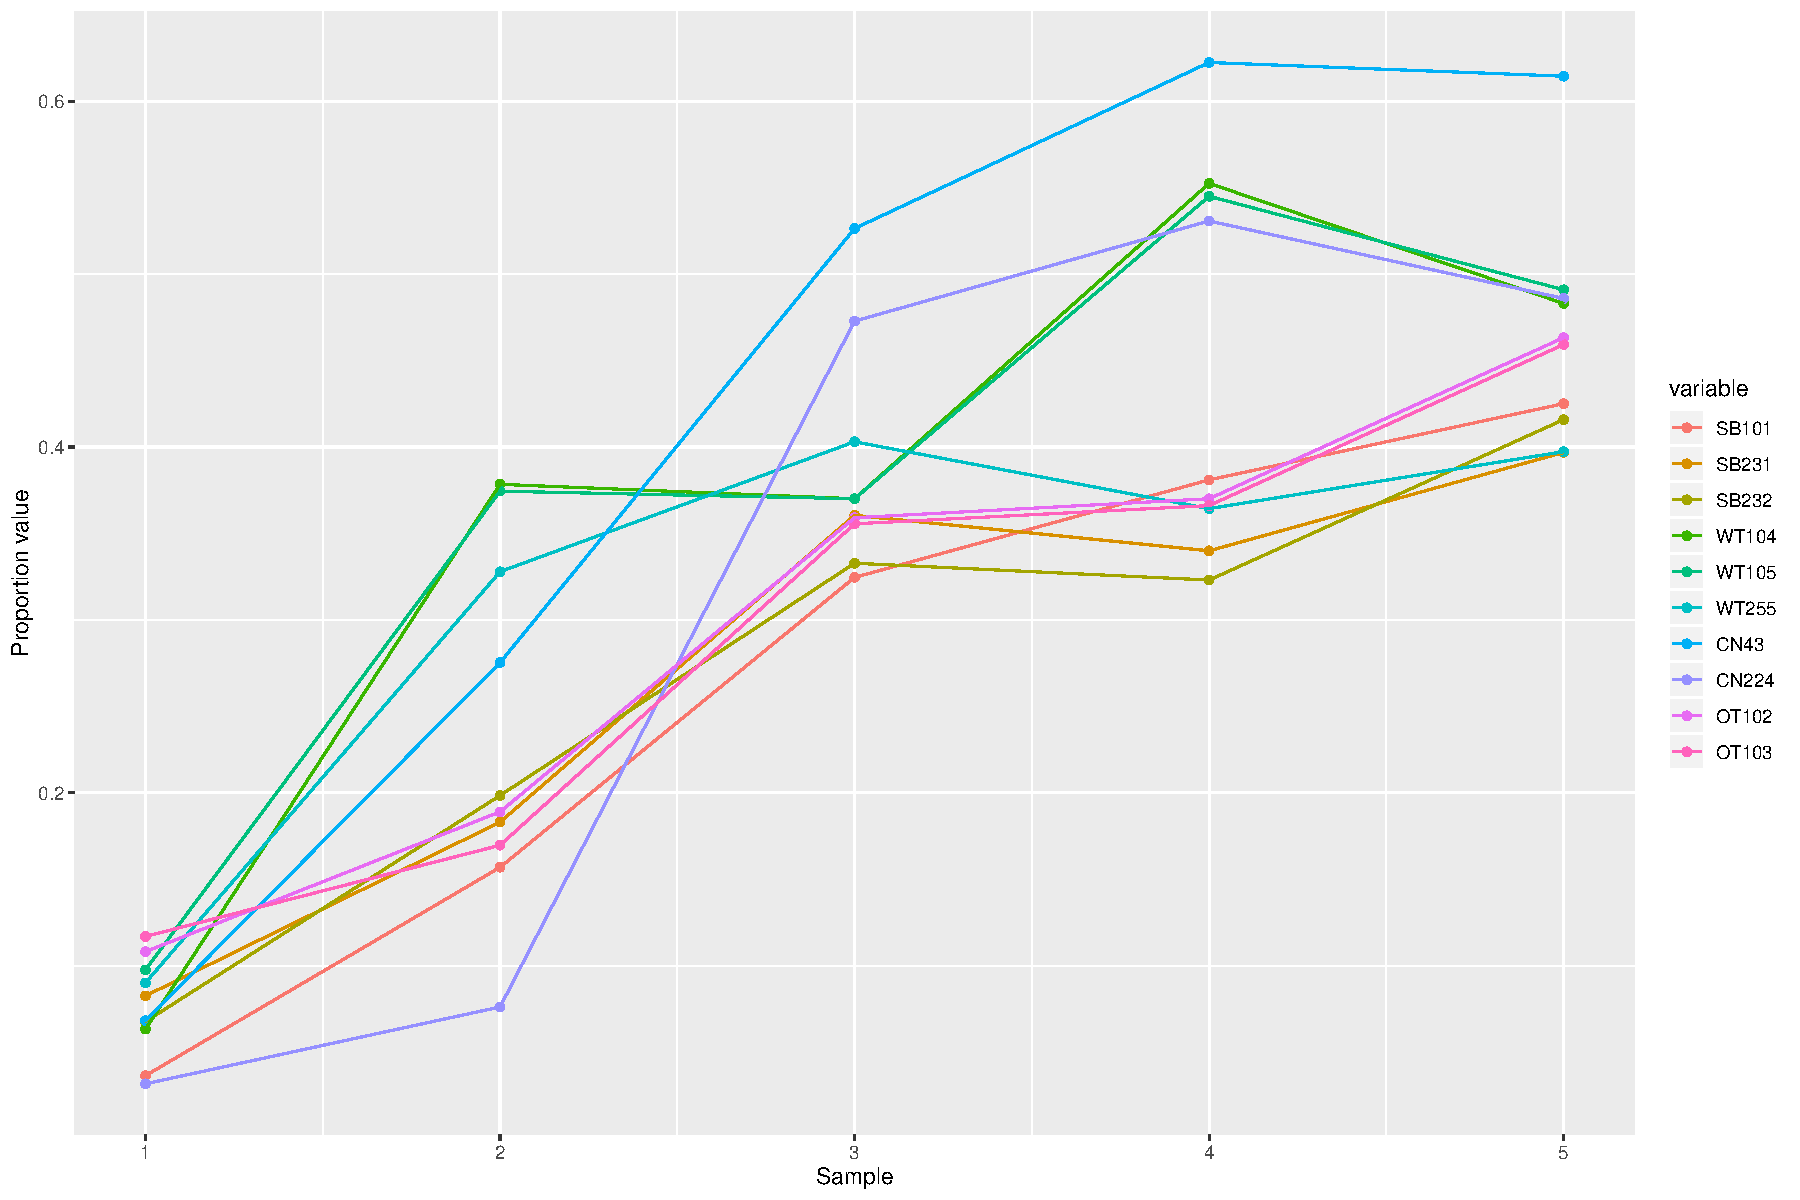
\includegraphics[width = .49\linewidth]{/Parameters/rv_proportion}}
\caption{Pixel proportions on the analyzed regions more similar to the trihedral and random volume as function of time, where SB, WT, CN and OT indicate, respectively, Soybeans, Wheat, Canola and Oats}
\label{fig:pixel_proportions}
\end{figure*}

\section{Fitting the Beta Distribution}

Figs.~\ref{fig:sb101_hist_tri} to~\ref{fig:ot103_hist_rv} show the histograms of the Geodesic Distances between the scatterer (random or trihedral volume) and the pixels of the sample most similar to it.
The number of those pixels are in Table~\ref{tab:size_sample}, in which TR and RV indicate, respectively, trihedral and random volume. 
The parameters of the Beta distribution were estimated by maximum likelihood.

Table~\ref{tab:pvalues_table} shows the $p$-values of the goodness-of-fit as assessed by the Komolgorov-Smirnov test. 
Largest and smallest $p$-values are highlighted in bold.

\begin{table}[hbt]
\centering
\caption{Number of pixels more similar to trihedral and random volume}\label{tab:size_sample}
\begin{tabular}{lrrrrrrrrrr}

\toprule
& \multicolumn{2}{c}{First} & \multicolumn{2}{c}{Second} & \multicolumn{2}{c}{Third} & \multicolumn{2}{c}{Fourth} & \multicolumn{2}{c}{Fifth}\\
& \multicolumn{2}{c}{observation} & \multicolumn{2}{c}{observation} & \multicolumn{2}{c}{observation} & \multicolumn{2}{c}{observation} & \multicolumn{2}{c}{observation}\\
& TR & RV & TR & RV & TR & RV & TR & RV& TR & RV\\
\cmidrule(lr){2-11}
\textbf{SB 101} & 1481 & 71 & 867 & 306 & 429 & 633 & 397 & 743 & 319 & 829\\
\textbf{SB 231} & 1285 & 148 & 656 & 381 & 449 & 706 & 615 & 649 & 508 & 775\\
\textbf{SB 232} & 1275 & 132 & 649 & 387 & 474 & 649 & 596 & 630 & 518 & 811\\
\textbf{WT 104} & 1618 & 144 & 478 & 861 & 161 & 842 & 133 & 1257 & 140 & 1099\\
\textbf{WT 105} & 1488 & 222 & 482 & 852 & 196 & 842 & 154 & 1240 & 160 & 1117\\
\textbf{WT 255} & 1552 & 205 & 567 & 746 & 180 & 917 & 85 & 829 & 157 & 904\\
\textbf{CN 43}  & 1964 & 155 & 1002 & 625 & 485 & 1195 & 168 & 1413 & 207 & 1395\\
\textbf{CN 224} & 2106 & 87 & 1716 & 209 & 234 & 1298 & 162 & 1457 & 212 & 1334\\
\textbf{OT 102} & 1441 & 246 & 1087 & 430 & 354 & 817 & 121 & 842 & 92 & 1054\\
\textbf{OT 103} & 1429 & 266 & 1153 & 386 & 388 & 806 & 110 & 833 & 99 & 1045\\
\bottomrule
\end{tabular} 
\end{table}


\begin{table}[hbt]
\centering
\caption{$p$-values of the Kolmogorov-Smirnov goodness-of-fit test of the distances to trihedral an random volume}\label{tab:pvalues_table}
\begin{tabular}{lrrrrrrrrrr}

\toprule
& \multicolumn{2}{c}{First} & \multicolumn{2}{c}{Second} & \multicolumn{2}{c}{Third} & \multicolumn{2}{c}{Fourth} & \multicolumn{2}{c}{Fifth}\\
& \multicolumn{2}{c}{observation} & \multicolumn{2}{c}{observation} & \multicolumn{2}{c}{observation} & \multicolumn{2}{c}{observation} & \multicolumn{2}{c}{observation}\\
& TR & RV & TR & RV & TR & RV & TR & RV& TR & RV\\
\cmidrule(lr){2-11}
\textbf{SB 101} & 0.065 & 0.517 & 0.947 & 0.758 & \textbf{0.059} & 0.495 & 0.452 & 0.109 & 0.401 & 0.144\\
\textbf{SB 231} & 0.775 & 0.242 & 0.573 & 0.166 & 0.314 & 0.275 & 0.239 & 0.114 & 0.416 & 0.070\\
\textbf{SB 232} & 0.244 & 0.340 & 0.968 & 0.328 & 0.713 & 0.070 & 0.422 & 0.357 & 0.163 & 0.630\\
\textbf{WT 104} & 0.178 & 0.715 & 0.421 & 0.094 & 0.514 & 0.779 & 0.062 & 0.369 & 0.602 & 0.919\\
\textbf{WT 105} & 0.231 & 0.090 & 0.069 & 0.139 & 0.557 & 0.613 & 0.108 & 0.195 & 0.192 & 0.252\\
\textbf{WT 255} & 0.235 & 0.513 & 0.270 & 0.375 & 0.628 & 0.279 & 0.653 & 0.069 & 0.437 & \textbf{0.993}\\
\textbf{CN 43}  & 0.238 & 0.406 & 0.217 & 0.202 & 0.930 & 0.318 & 0.623 & 0.732 & 0.262 & 0.747\\
\textbf{CN 224} & 0.184 & 0.116 & 0.128 & 0.333 & 0.298 & 0.714 & 0.813 & 0.409 & 0.305 & 0.391\\
\textbf{OT 102} & 0.289 & 0.191 & 0.243 & 0.532 & 0.384 & 0.212 & 0.710 & 0.370 & 0.928 & 0.396\\
\textbf{OT 103} & 0.096 & 0.139 & 0.139 & 0.186 & 0.265 & 0.079 & 0.936 & 0.079 & 0.989 & 0.489\\
\bottomrule
\end{tabular} 
\end{table}

%SB101
\begin{figure*}[hbt]
\centering
\subfigure[1th observation]{\includegraphics[width = .49\linewidth]{/Histograms/1th_observation/Soybeans_101/histogram_trihedral_1}}
\subfigure[2th observation]{\includegraphics[width = .49\linewidth]{/Histograms/2th_observation/Soybeans_101/histogram_trihedral_2}}
\subfigure[3th observation]{\includegraphics[width = .49\linewidth]{/Histograms/3th_observation/Soybeans_101/histogram_trihedral_3}}
\subfigure[4th observation]{\includegraphics[width = .49\linewidth]{/Histograms/4th_observation/Soybeans_101/histogram_trihedral_4}}
\subfigure[5th observation]{\includegraphics[width = .49\linewidth]{/Histograms/5th_observation/Soybeans_101/histogram_trihedral_5}}
\caption{Histograms of the Geodesic Distances between trihedral and the pixels of the sample extracted from Soybeans 101 most similar to trihedral}
\label{fig:sb101_hist_tri}
\end{figure*}

\begin{figure*}[hbt]
\centering
\subfigure[1th observation]{\includegraphics[width = .49\linewidth]{/Histograms/1th_observation/Soybeans_101/histogram_random_volume_1}}
\subfigure[2th observation]{\includegraphics[width = .49\linewidth]{/Histograms/2th_observation/Soybeans_101/histogram_random_volume_2}}
\subfigure[3th observation]{\includegraphics[width = .49\linewidth]{/Histograms/3th_observation/Soybeans_101/histogram_random_volume_3}}
\subfigure[4th observation]{\includegraphics[width = .49\linewidth]{/Histograms/4th_observation/Soybeans_101/histogram_random_volume_4}}
\subfigure[5th observation]{\includegraphics[width = .49\linewidth]{/Histograms/5th_observation/Soybeans_101/histogram_random_volume_5}}
\caption{Histograms of the Geodesic Distances between random volume and the pixels of the sample extracted from Soybeans 101 most similar to random volume}
\label{fig:sb101_hist_rv}
\end{figure*}

%SB231
\begin{figure*}[hbt]
\centering
\subfigure[1th observation]{\includegraphics[width = .49\linewidth]{/Histograms/1th_observation/Soybeans_231/histogram_trihedral_1}}
\subfigure[2th observation]{\includegraphics[width = .49\linewidth]{/Histograms/2th_observation/Soybeans_231/histogram_trihedral_2}}
\subfigure[3th observation]{\includegraphics[width = .49\linewidth]{/Histograms/3th_observation/Soybeans_231/histogram_trihedral_3}}
\subfigure[4th observation]{\includegraphics[width = .49\linewidth]{/Histograms/4th_observation/Soybeans_231/histogram_trihedral_4}}
\subfigure[5th observation]{\includegraphics[width = .49\linewidth]{/Histograms/5th_observation/Soybeans_231/histogram_trihedral_5}}
\caption{Histograms of the Geodesic Distances between trihedral and the pixels of the sample extracted from Soybeans 231 most similar to trihedral}
\label{fig:sb231_hist_tri}
\end{figure*}

\begin{figure*}[hbt]
\centering
\subfigure[1th observation]{\includegraphics[width = .49\linewidth]{/Histograms/1th_observation/Soybeans_231/histogram_random_volume_1}}
\subfigure[2th observation]{\includegraphics[width = .49\linewidth]{/Histograms/2th_observation/Soybeans_231/histogram_random_volume_2}}
\subfigure[3th observation]{\includegraphics[width = .49\linewidth]{/Histograms/3th_observation/Soybeans_231/histogram_random_volume_3}}
\subfigure[4th observation]{\includegraphics[width = .49\linewidth]{/Histograms/4th_observation/Soybeans_231/histogram_random_volume_4}}
\subfigure[5th observation]{\includegraphics[width = .49\linewidth]{/Histograms/5th_observation/Soybeans_231/histogram_random_volume_5}}
\caption{Histograms of the Geodesic Distances between random volume and the pixels of the sample extracted from Soybeans 231 most similar to random volume}
\label{fig:sb231_hist_rv}
\end{figure*}

%SB232
\begin{figure*}[hbt]
\centering
\subfigure[1th observation]{\includegraphics[width = .49\linewidth]{/Histograms/1th_observation/Soybeans_232/histogram_trihedral_1}}
\subfigure[2th observation]{\includegraphics[width = .49\linewidth]{/Histograms/2th_observation/Soybeans_232/histogram_trihedral_2}}
\subfigure[3th observation]{\includegraphics[width = .49\linewidth]{/Histograms/3th_observation/Soybeans_232/histogram_trihedral_3}}
\subfigure[4th observation]{\includegraphics[width = .49\linewidth]{/Histograms/4th_observation/Soybeans_232/histogram_trihedral_4}}
\subfigure[5th observation]{\includegraphics[width = .49\linewidth]{/Histograms/5th_observation/Soybeans_232/histogram_trihedral_5}}
\caption{Histograms of the Geodesic Distances between trihedral and the pixels of the sample extracted from Soybeans 232 most similar to trihedral}
\label{fig:sb232_hist_tri}
\end{figure*}

\begin{figure*}[hbt]
\centering
\subfigure[1th observation]{\includegraphics[width = .49\linewidth]{/Histograms/1th_observation/Soybeans_232/histogram_random_volume_1}}
\subfigure[2th observation]{\includegraphics[width = .49\linewidth]{/Histograms/2th_observation/Soybeans_232/histogram_random_volume_2}}
\subfigure[3th observation]{\includegraphics[width = .49\linewidth]{/Histograms/3th_observation/Soybeans_232/histogram_random_volume_3}}
\subfigure[4th observation]{\includegraphics[width = .49\linewidth]{/Histograms/4th_observation/Soybeans_232/histogram_random_volume_4}}
\subfigure[5th observation]{\includegraphics[width = .49\linewidth]{/Histograms/5th_observation/Soybeans_232/histogram_random_volume_5}}
\caption{Histograms of the Geodesic Distances between random volume and the pixels of the sample extracted from Soybeans 232 most similar to random volume}
\label{fig:sb232_hist_rv}
\end{figure*}

%WT104
\begin{figure*}[hbt]
\centering
\subfigure[1th observation]{\includegraphics[width = .49\linewidth]{/Histograms/1th_observation/Wheat_104/histogram_trihedral_1}}
\subfigure[2th observation]{\includegraphics[width = .49\linewidth]{/Histograms/2th_observation/Wheat_104/histogram_trihedral_2}}
\subfigure[3th observation]{\includegraphics[width = .49\linewidth]{/Histograms/3th_observation/Wheat_104/histogram_trihedral_3}}
\subfigure[4th observation]{\includegraphics[width = .49\linewidth]{/Histograms/4th_observation/Wheat_104/histogram_trihedral_4}}
\subfigure[5th observation]{\includegraphics[width = .49\linewidth]{/Histograms/5th_observation/Wheat_104/histogram_trihedral_5}}
\caption{Histograms of the Geodesic Distances between trihedral and the pixels of the sample extracted from Wheat 104 most similar to trihedral}
\label{fig:wt104_hist_tri}
\end{figure*}

\begin{figure*}[hbt]
\centering
\subfigure[1th observation]{\includegraphics[width = .49\linewidth]{/Histograms/1th_observation/Wheat_104/histogram_random_volume_1}}
\subfigure[2th observation]{\includegraphics[width = .49\linewidth]{/Histograms/2th_observation/Wheat_104/histogram_random_volume_2}}
\subfigure[3th observation]{\includegraphics[width = .49\linewidth]{/Histograms/3th_observation/Wheat_104/histogram_random_volume_3}}
\subfigure[4th observation]{\includegraphics[width = .49\linewidth]{/Histograms/4th_observation/Wheat_104/histogram_random_volume_4}}
\subfigure[5th observation]{\includegraphics[width = .49\linewidth]{/Histograms/5th_observation/Wheat_104/histogram_random_volume_5}}
\caption{Histograms of the Geodesic Distances between random volume and the pixels of the sample extracted from Wheat 104 most similar to random volume}
\label{fig:wt104_hist_rv}
\end{figure*}

%WT105
\begin{figure*}[hbt]
\centering
\subfigure[1th observation]{\includegraphics[width = .49\linewidth]{/Histograms/1th_observation/Wheat_105/histogram_trihedral_1}}
\subfigure[2th observation]{\includegraphics[width = .49\linewidth]{/Histograms/2th_observation/Wheat_105/histogram_trihedral_2}}
\subfigure[3th observation]{\includegraphics[width = .49\linewidth]{/Histograms/3th_observation/Wheat_105/histogram_trihedral_3}}
\subfigure[4th observation]{\includegraphics[width = .49\linewidth]{/Histograms/4th_observation/Wheat_105/histogram_trihedral_4}}
\subfigure[5th observation]{\includegraphics[width = .49\linewidth]{/Histograms/5th_observation/Wheat_105/histogram_trihedral_5}}
\caption{Histograms of the Geodesic Distances between trihedral and the pixels of the sample extracted from Wheat 105 most similar to trihedral}
\label{fig:wt105_hist_tri}
\end{figure*}

\begin{figure*}[hbt]
\centering
\subfigure[1th observation]{\includegraphics[width = .49\linewidth]{/Histograms/1th_observation/Wheat_105/histogram_random_volume_1}}
\subfigure[2th observation]{\includegraphics[width = .49\linewidth]{/Histograms/2th_observation/Wheat_105/histogram_random_volume_2}}
\subfigure[3th observation]{\includegraphics[width = .49\linewidth]{/Histograms/3th_observation/Wheat_105/histogram_random_volume_3}}
\subfigure[4th observation]{\includegraphics[width = .49\linewidth]{/Histograms/4th_observation/Wheat_105/histogram_random_volume_4}}
\subfigure[5th observation]{\includegraphics[width = .49\linewidth]{/Histograms/5th_observation/Wheat_105/histogram_random_volume_5}}
\caption{Histograms of the Geodesic Distances between random volume and the pixels of the sample extracted from Wheat 105 most similar to random volume}
\label{fig:wt105_hist_rv}
\end{figure*}

%WT255
\begin{figure*}[hbt]
\centering
\subfigure[1th observation]{\includegraphics[width = .49\linewidth]{/Histograms/1th_observation/Wheat_225/histogram_trihedral_1}}
\subfigure[2th observation]{\includegraphics[width = .49\linewidth]{/Histograms/2th_observation/Wheat_225/histogram_trihedral_2}}
\subfigure[3th observation]{\includegraphics[width = .49\linewidth]{/Histograms/3th_observation/Wheat_225/histogram_trihedral_3}}
\subfigure[4th observation]{\includegraphics[width = .49\linewidth]{/Histograms/4th_observation/Wheat_225/histogram_trihedral_4}}
\subfigure[5th observation]{\includegraphics[width = .49\linewidth]{/Histograms/5th_observation/Wheat_225/histogram_trihedral_5}}
\caption{Histograms of the Geodesic Distances between trihedral and the pixels of the sample extracted from Wheat 225 most similar to trihedral}
\label{fig:wt255_hist_tri}
\end{figure*}

\begin{figure*}[hbt]
\centering
\subfigure[1th observation]{\includegraphics[width = .49\linewidth]{/Histograms/1th_observation/Wheat_225/histogram_random_volume_1}}
\subfigure[2th observation]{\includegraphics[width = .49\linewidth]{/Histograms/2th_observation/Wheat_225/histogram_random_volume_2}}
\subfigure[3th observation]{\includegraphics[width = .49\linewidth]{/Histograms/3th_observation/Wheat_225/histogram_random_volume_3}}
\subfigure[4th observation]{\includegraphics[width = .49\linewidth]{/Histograms/4th_observation/Wheat_225/histogram_random_volume_4}}
\subfigure[5th observation]{\includegraphics[width = .49\linewidth]{/Histograms/5th_observation/Wheat_225/histogram_random_volume_5}}
\caption{Histograms of the Geodesic Distances between random volume and the pixels of the sample extracted from Wheat 225 most similar to random volume}
\label{fig:wt255_hist_rv}
\end{figure*}

%CN43
\begin{figure*}[hbt]
\centering
\subfigure[1th observation]{\includegraphics[width = .49\linewidth]{/Histograms/1th_observation/Canola_43/histogram_trihedral_1}}
\subfigure[2th observation]{\includegraphics[width = .49\linewidth]{/Histograms/2th_observation/Canola_43/histogram_trihedral_2}}
\subfigure[3th observation]{\includegraphics[width = .49\linewidth]{/Histograms/3th_observation/Canola_43/histogram_trihedral_3}}
\subfigure[4th observation]{\includegraphics[width = .49\linewidth]{/Histograms/4th_observation/Canola_43/histogram_trihedral_4}}
\subfigure[5th observation]{\includegraphics[width = .49\linewidth]{/Histograms/5th_observation/Canola_43/histogram_trihedral_5}}
\caption{Histograms of the Geodesic Distances between trihedral and the pixels of the sample extracted from Canola 43 most similar to trihedral}
\label{fig:cn43_hist_tri}
\end{figure*}

\begin{figure*}[hbt]
\centering
\subfigure[1th observation]{\includegraphics[width = .49\linewidth]{/Histograms/1th_observation/Canola_43/histogram_random_volume_1}}
\subfigure[2th observation]{\includegraphics[width = .49\linewidth]{/Histograms/2th_observation/Canola_43/histogram_random_volume_2}}
\subfigure[3th observation]{\includegraphics[width = .49\linewidth]{/Histograms/3th_observation/Canola_43/histogram_random_volume_3}}
\subfigure[4th observation]{\includegraphics[width = .49\linewidth]{/Histograms/4th_observation/Canola_43/histogram_random_volume_4}}
\subfigure[5th observation]{\includegraphics[width = .49\linewidth]{/Histograms/5th_observation/Canola_43/histogram_random_volume_5}}
\caption{Histograms of the Geodesic Distances between random volume and the pixels of the sample extracted from Canola 43 most similar to random volume}
\label{fig:cn43_hist_rv}
\end{figure*}

%CN224
\begin{figure*}[hbt]
\centering
\subfigure[1th observation]{\includegraphics[width = .49\linewidth]{/Histograms/1th_observation/Canola_224/histogram_trihedral_1}}
\subfigure[2th observation]{\includegraphics[width = .49\linewidth]{/Histograms/2th_observation/Canola_224/histogram_trihedral_2}}
\subfigure[3th observation]{\includegraphics[width = .49\linewidth]{/Histograms/3th_observation/Canola_224/histogram_trihedral_3}}
\subfigure[4th observation]{\includegraphics[width = .49\linewidth]{/Histograms/4th_observation/Canola_224/histogram_trihedral_4}}
\subfigure[5th observation]{\includegraphics[width = .49\linewidth]{/Histograms/5th_observation/Canola_224/histogram_trihedral_5}}
\caption{Histograms of the Geodesic Distances between trihedral and the pixels of the sample extracted from Canola 224 most similar to trihedral}
\label{fig:cn224_hist_tri}
\end{figure*}

\begin{figure*}[hbt]
\centering
\subfigure[1th observation]{\includegraphics[width = .49\linewidth]{/Histograms/1th_observation/Canola_224/histogram_random_volume_1}}
\subfigure[2th observation]{\includegraphics[width = .49\linewidth]{/Histograms/2th_observation/Canola_224/histogram_random_volume_2}}
\subfigure[3th observation]{\includegraphics[width = .49\linewidth]{/Histograms/3th_observation/Canola_224/histogram_random_volume_3}}
\subfigure[4th observation]{\includegraphics[width = .49\linewidth]{/Histograms/4th_observation/Canola_224/histogram_random_volume_4}}
\subfigure[5th observation]{\includegraphics[width = .49\linewidth]{/Histograms/5th_observation/Canola_224/histogram_random_volume_5}}
\caption{Histograms of the Geodesic Distances between random volume and the pixels of the sample extracted from Canola 224 most similar to random volume}
\label{fig:cn224_hist_rv}
\end{figure*}

%OT102
\begin{figure*}[hbt]
\centering
\subfigure[1th observation]{\includegraphics[width = .49\linewidth]{/Histograms/1th_observation/Oats_102/histogram_trihedral_1}}
\subfigure[2th observation]{\includegraphics[width = .49\linewidth]{/Histograms/2th_observation/Oats_102/histogram_trihedral_2}}
\subfigure[3th observation]{\includegraphics[width = .49\linewidth]{/Histograms/3th_observation/Oats_102/histogram_trihedral_3}}
\subfigure[4th observation]{\includegraphics[width = .49\linewidth]{/Histograms/4th_observation/Oats_102/histogram_trihedral_4}}
\subfigure[5th observation]{\includegraphics[width = .49\linewidth]{/Histograms/5th_observation/Oats_102/histogram_trihedral_5}}
\caption{Histograms of the Geodesic Distances between trihedral and the pixels of the sample extracted from Oats 102 most similar to trihedral}
\label{fig:ot102_hist_tri}
\end{figure*}

\begin{figure*}[hbt]
\centering
\subfigure[1th observation]{\includegraphics[width = .49\linewidth]{/Histograms/1th_observation/Oats_102/histogram_random_volume_1}}
\subfigure[2th observation]{\includegraphics[width = .49\linewidth]{/Histograms/2th_observation/Oats_102/histogram_random_volume_2}}
\subfigure[3th observation]{\includegraphics[width = .49\linewidth]{/Histograms/3th_observation/Oats_102/histogram_random_volume_3}}
\subfigure[4th observation]{\includegraphics[width = .49\linewidth]{/Histograms/4th_observation/Oats_102/histogram_random_volume_4}}
\subfigure[5th observation]{\includegraphics[width = .49\linewidth]{/Histograms/5th_observation/Oats_102/histogram_random_volume_5}}
\caption{Histograms of the Geodesic Distances between random volume and the pixels of the sample extracted from Oats 102 most similar to random volume}
\label{fig:ot102_hist_rv}
\end{figure*}

%OT103
\begin{figure*}[hbt]
\centering
\subfigure[1th observation]{\includegraphics[width = .49\linewidth]{/Histograms/1th_observation/Oats_103/histogram_trihedral_1}}
\subfigure[2th observation]{\includegraphics[width = .49\linewidth]{/Histograms/2th_observation/Oats_103/histogram_trihedral_2}}
\subfigure[3th observation]{\includegraphics[width = .49\linewidth]{/Histograms/3th_observation/Oats_103/histogram_trihedral_3}}
\subfigure[4th observation]{\includegraphics[width = .49\linewidth]{/Histograms/4th_observation/Oats_103/histogram_trihedral_4}}
\subfigure[5th observation]{\includegraphics[width = .49\linewidth]{/Histograms/5th_observation/Oats_103/histogram_trihedral_5}}
\caption{Histograms of the Geodesic Distances between trihedral and the pixels of the sample extracted from Oats 103 most similar to trihedral}
\label{fig:ot103_hist_tri}
\end{figure*}

\begin{figure*}[hbt]
\centering
\subfigure[1th observation]{\includegraphics[width = .49\linewidth]{/Histograms/1th_observation/Oats_103/histogram_random_volume_1}}
\subfigure[2th observation]{\includegraphics[width = .49\linewidth]{/Histograms/2th_observation/Oats_103/histogram_random_volume_2}}
\subfigure[3th observation]{\includegraphics[width = .49\linewidth]{/Histograms/3th_observation/Oats_103/histogram_random_volume_3}}
\subfigure[4th observation]{\includegraphics[width = .49\linewidth]{/Histograms/4th_observation/Oats_103/histogram_random_volume_4}}
\subfigure[5th observation]{\includegraphics[width = .49\linewidth]{/Histograms/5th_observation/Oats_103/histogram_random_volume_5}}
\caption{Histograms of the Geodesic Distances between random volume and the pixels of the sample extracted from Oats 103 most similar to random volume}
\label{fig:ot103_hist_rv}
\end{figure*}

\section{Parameters evaluation}
When observing the regions referring to Soybeans 231 and 232 along its samples in the Fig.~\ref{fig:regions}, which are respectively indexed by 2 and 3, it can be assumed that there was a gradual increase in the degree of vegetation of these regions.

In order to relate this to the variation of the information contained in the distances of the data to the trihedral scatterer, in Figs.~\ref{subfig:tri_mean_sb231} and~\ref{subfig:tri_mean_sb232} we show, for each observation, a boxplot of the means of the distances between trihedral and the subregions generated by dividing a region into 45 subregions of size $7\times 6$.
In addition, all boxplots were connected by the mean of their means.

We adjusted the mean as a function of time for both regions with the following function:
\begin{equation}
f(t) = -\frac{a}{bt + c} + d,
\end{equation}
in which $a = 4.741$, $b = 2.415$, $c = 67.565$, $d = 0.276$ and $t$ is the number of days since the first observation ($t = 0$). 
We checked lack of fit with ANOVA; Tables~\ref{tab:anova_sb231} and~\ref{tab:anova_sb232} show the results. 
We conclude that the proposed model is acceptable at the significance level of $0.1$.

\begin{table}[hbt]
  \centering
  \caption{ANOVA for lack of fit on Soybeans 231}
  \label{tab:anova_sb231}
  \begin{tabular}{lrrrrr}
    \toprule
    & Degree of & Sum of squared & Mean squared & Fisher & p-value\\
    & freedom & errors & error & statistics &\\
    \cmidrule(lr){2-6}
    \textbf{Residual} & 223 & 0.1912 & 0.0008 & &\\
    \textbf{Lack od fit} & 3 & 0.0043 & 0.0014 & 1.7087 & 0.1661\\
    \textbf{Pure error} & 220 & 0.1859 & 0.0008 & &\\
    \bottomrule
  \end{tabular}
\end{table}

\begin{table}[hbt]
  \centering
  \caption{ANOVA for lack of fit on Soybeans 232}
  \label{tab:anova_sb232}
  \begin{tabular}{lrrrrr}
    \toprule
    & Degree of & Sum of squared & Mean squared & Fisher & p-value\\
    & freedom & errors & error & statistics &\\
    \cmidrule(lr){2-6}
    \textbf{Residual} & 223 & 0.1836 & 0.0008 & &\\
    \textbf{Lack od fit} & 3 & 0.0020 & 0.0007 & 0.7973 & 0.4965\\
    \textbf{Pure error} & 220 & 0.1819 & 0.0008 & &\\
    \bottomrule
  \end{tabular}
\end{table}

\begin{figure*}[hbt]
  \subfigure[Soybeans 231\label{subfig:tri_mean_sb231}]{\includegraphics[width = .5\linewidth]{/Parameters/mean_tri_over_time_sb231}}
  \subfigure[Soybeans 232\label{subfig:tri_mean_sb232}]{\includegraphics[width = .5\linewidth]{/Parameters/mean_tri_over_time_sb232}}
  \caption{Mean of the distances between trihedral and samples extracted from Soybeans 231 and 232 over time}
  \label{fig:tri_mean_sb_231_232}
\end{figure*}

\section{Classifier for vegetation regions}

We propose a classifier based on results of the analysis of a subregion of Soybeans 231 with dimensions $15\times 15$ pixels. 
We fitted a Beta distribution to its geodesic distances to the left and right helices on the first and last observation of this subregion, which belong to the regions indicated by index 1 in the figures \ref{fig:r1} and \ref{fig:r5}, respectively. 
%%% ACF Não ficou claro. O que são estas "first and last observation".
%%% DFC Corrigido

Figs.~\ref{subfig:lh_subreg_sb231} and~\ref{subfig:lh_subreg_sb231} show the histograms and the fitted densities. 
%%% ACF veja acima como escrevi um texto similar para o que segue 
In adiction, the Komolgorov-Smirnov test for goodness-of-fit was performed and returned $p$-values are in the table \ref{tab:pvalues_table_lh_rh}.

\begin{figure*}[hbt]
  \subfigure[Histogram of the distances to left helix\label{subfig:lh_subreg_sb231}]{\includegraphics[width = .5\linewidth]{/Histograms/hist_sb231_lh}}
  \subfigure[Histogram of the distances to right helix\label{subfig:rh_subreg_sb231}]{\includegraphics[width = .5\linewidth]{/Histograms/hist_sb231_rh}}
  \caption{Histograms of the distances between subregion extracted from Soybeans 231 and elementary scatterers}
  \label{fig:hist_lh_rh}
\end{figure*}

\begin{table}[hbt]
  \centering
  \caption{$p$-values of the Kolmogorov-Smirnov goodness-of-fit test of the distances to left and right helix}\label{tab:pvalues_table_lh_rh}
  \begin{tabular}{lrr}
    \toprule
    & Left helix & Right helix\\
    \cmidrule{2-3}
    \textbf{First sample} & 0.406 & 0.172\\
    \textbf{Last sample} & 0.940 & 0.817\\
    \bottomrule
  \end{tabular}
\end{table}

Since the distances to the left helix and right helix are independent, because these are orthogonal, it is possible to define $d = 0.912$ as cutoff point for the densities Beta(21, 1.6) and Beta(10, 1.85) and obtain the joint probabilities shown in the table \ref{tab:joint_prob}, where $D_{lh}$ and $D_{rh}$ are respectively the distance to left helix and right helix.  These joint probabilities allow evaluate the error related in the separation of populations by this cutoff point.

\begin{table}[hbt]
  \centering
  \caption{Joint probabilities for distance to left and right helix}\label{tab:joint_prob}
  \begin{tabular*}{\textwidth}{l@{\extracolsep{\fill}}cccc}
    \toprule
    & \multicolumn{2}{c}{$D_{rh} \le 0.912$} & \multicolumn{2}{c}{$D_{rh} > 0.912$}\\
    & $D_{rh} \le 0.912$ & $D_{rh} > 0.912$ & $D_{rh} \le 0.912$ & $D_{rh} > 0.912$\\
    \cmidrule{2-5}
    \textbf{First sample} & \textbf{0.09} & 0.21 & 0.21 & \textbf{0.49}\\
    \textbf{Last sample} & \textbf{0.49} & 0.21 & 0.21 & \textbf{0.09}\\
    \bottomrule
  \end{tabular*}
\end{table}

Assume that the pixels in the first and last observation as poor and rich in vegetation, respectively. 
Then, it is possible classify pixels with $d_{lh} > 0.912$ and $d_{rh} > 0.912$ as poor in vegetation and those with $d_{lh} \le 0.912$ and $d_{rh} \le 0.912$ as rich in vegetation. 
By this rule, there is $0.09$ probability that a poor pixel in vegetation be classified rich and vice-versa. 
However, this approach allows classifying only \SI{56}{\percent} of both populations.

%%% ACF Até aqui 3 Outubro 2019, 9:05 GMT+8
%%% ACF Use \SI{44}{\percent} para porcentagens
For classify the other \SI{44}{\percent} of the population, the components of the data in the direction of these elementary scatterers are removed as follows:
%%% ACF Use \rangle e \langle para produto interno
\begin{equation}
  v_{data}' =  v_{data} - \frac{\langle v_{data}, v_{lh} \rangle}{\norm{v_{lh}}^2} v_{lh} - \frac{\langle v_{data}, v_{rh} \rangle}{\norm{v_{rh}}^2} v_{rh},
\end{equation}
where $v_{data}$, $v_{lh}$ and $v_{rh}$ are respectively data, left helix and right helix in Kennaugh form. Then, the follow distance is calculate:
\begin{equation}
  D_{d}' = \frac{1}{\pi} \cos^{-1}\left(\frac{\langle v_{data}', v_d \rangle}{\norm{v_{data}'}\norm{v_d}}\right) = \frac{1}{2}GD(v_{data}', v_d),
\end{equation}
where $D_d' \in [0, 1]$ and $v_d$ is dihedral elementary scatterer in Kennaugh form. This distance was used because $GD(v_{data}', v_d) \in [0, 2]$ for analysed subregion. The histograms of this distance between dihedral and analysed samples are shown in the figure \ref{fig:hist_di} and the $p$-values from Komolgorov-Smirnov goodness-of-fit test for first and last observation are respectively $0.127$ and $0.105$. 
\begin{figure*}[hbt]
  \centering
  \includegraphics[width = .5\linewidth]{Histograms/hist_mod_di}
  \caption{Modified geodesic distance between dihedral and samples}
  \label{fig:hist_di}
\end{figure*}

Since the procedure described makes $D_d'$ independent of $D_{lh}$ and $D_{rh}$, the fitted distributions can be used to classify the remaining population. For this, 
define $d_d = 0.462$ and $d_d = 0.512$, which are inserctions between densities, as cutoff points, whose related probabilities are shown in the table \ref{tab:prob_di}.
With this, a pixel unclassified by $d_{lh}$ and $d_{rh}$ and with $d_d' < 0.462$ or $d_d' > 0.512$ can be classified as rich in vegetation and, in opposite case, as poor in vegetation. In this situation, the probability of classify a poor pixel as rich is 0.13 and the opposite with probability 0.44. 

\begin{table}[hbt]
  \centering
  \caption{Probabilities for modified geodesic distance to dihedral}\label{tab:prob_di}
  \begin{tabular*}{\textwidth}{l@{\extracolsep{\fill}}ccc}
    \toprule
    & $D_d' < 0.462$ & $0.462 \le D_d' \le 0.512$ & $D_d' > 0.512$\\
    \cmidrule{2-4}
    \textbf{First sample} & 0.05 & 0.87 & 0.08\\
    \textbf{Last sample} & 0.21 & 0.44 & 0.35\\
    \bottomrule
  \end{tabular*}
\end{table}

This classifier can be evaluated by analysing of your confusion matrix. The table \ref{tab:theoretical_confusion_matrix} shows the theoretical confusion matrix (in percentage) for this model and the table \ref{tab:theoretical_analysis} shows the corresponding values of accuracy, coverage and precision.

\begin{table}[hbt]
  \centering
  \caption{Theoretical confusion matrix}\label{tab:theoretical_confusion_matrix}
  \begin{tabular}{lcc}
    \toprule
    & Poor in vegetation & Rich in vegetation\\
    \cmidrule{2-3}
    \textbf{Poor in vegetation} & 0.855 & 0.145\\
    \textbf{Rich in vegetation} & 0.275 & 0.725\\
    \bottomrule
  \end{tabular}
\end{table}

\begin{table}[hbt]
  \centering
  \caption{Theoretical accuracy, coverage and precision}\label{tab:theoretical_analysis}
  \begin{tabular}{lccc}
    \toprule
    & Accuracy & Coverage & Precision\\
    \cmidrule{2-4}
    \textbf{Poor in vegetation} & 0.790 & 0.855 & 0.757\\
    \textbf{Rich in vegetation} & 0.790 & 0.725 & 0.833\\
    \bottomrule
  \end{tabular}
\end{table}

The tables \ref{tab:subregion_sb231_confusion_matrix} and \ref{tab:sb231_confusion_matrix} show respectively the confusion matrices (in percentage) obtained by applying the model to the samples from the analysed subregion and Soybeans 231 region. In addiction, the tables \ref{tab:subregion_sb231_analysis} and \ref{tab:sb231_analysis} show their corresponding values of accuracy, coverage and precision. When comparing the theoretical values with the values obtained by applying the classifier to the data in these tables, the proximity between them is evident, which suggests that the model is suitable for the data.

\begin{table}[hbt]
  \centering
  \caption{Confusion matrix obtained by applying the model to the analysed subregion of Soybeans 231}\label{tab:subregion_sb231_confusion_matrix}
  \begin{tabular}{lcc}
    \toprule
    & Poor in vegetation & Rich in vegetation\\
    \cmidrule{2-3}
    \textbf{Poor in vegetation} & 0.827 & 0.173\\
    \textbf{Rich in vegetation} & 0.333 & 0.667\\
    \bottomrule
  \end{tabular}
\end{table}

\begin{table}[hbt]
  \centering
  \caption{Confusion matrix obtained by applying the model to the Soybeans 231 region}\label{tab:sb231_confusion_matrix}
  \begin{tabular}{lcc}
    \toprule
    & Poor in vegetation & Rich in vegetation\\
    \cmidrule{2-3}
    \textbf{Poor in vegetation} & 0.788 & 0.212\\
    \textbf{Rich in vegetation} & 0.333 & 0.667\\
    \bottomrule
  \end{tabular}
\end{table}

\begin{table}[hbt]
  \centering
  \caption{Accuracy, coverage and precision for the model applied to the analysed subregion}\label{tab:subregion_sb231_analysis}
  \begin{tabular}{lccc}
    \toprule
    & Accuracy & Coverage & Precision\\
    \cmidrule{2-4}
    \textbf{Poor in vegetation} & 0.747 & 0.827 & 0.713\\
    \textbf{Rich in vegetation} & 0.747 & 0.667 & 0.794\\
    \bottomrule
  \end{tabular}
\end{table}

\begin{table}[hbt]
  \centering
  \caption{Accuracy, coverage and precision for the model applied to the Soyebeans 231 region}\label{tab:sb231_analysis}
  \begin{tabular}{lccc}
    \toprule
    & Accuracy & Coverage & Precision\\
    \cmidrule{2-4}
    \textbf{Poor in vegetation} & 0.727 & 0.788 & 0.703\\
    \textbf{Rich in vegetation} & 0.727 & 0.667 & 0.759\\
    \bottomrule
  \end{tabular}
\end{table}

% \section{Conclusions}
% It can be concluded from the $p$-values table that the Beta distribution adjusts the distances of PolSAR data of the analyzed cultures to trihedral and random volume at the significance level of 0.05.

\end{document}